%%%%%%%%%%%%%%%%%%%%%%%%%%%%%%%%%%%%%%%%%%%%%%%%%%%%%%
%
% This file defines the style for your report
% You don't need to edit it any more, if not to change the authors name.
%
% Search below for the keyword:   GROUP
% insert your group number
%
% Search below for the keyword:   AUTHORS
% insert the name of the authors
%
% If you want to compile your document you have TWO ways
% depending on the fact that 
% 	1) you have inserted only postscript images in your .tex file 
%		---> then go to MODE 1
%	2) you have inserted other kind of images (jpg, pdf, ...) in your .tex file
%		---> then go to MODE 2
%
% MODE 1 
% Type:
% 	latex homebook.tex
%
% If the compilation runs successfully and you want to see the results type:
% 	xdvi homebook.dvi &
% and use the menus to go through the document
%
% If you want to create a pdf type:
% 	dvipdfm homebook.dvi
%
% a homebook.pdf file is created
% you can see it using the command:
% 	acroread homebook.pdf &
%
%
% MODE 2
% Type:
%	pdflatex homebook.tex
%
% If the compilation runs successfully you directly have the pdf file
% and you can see it using the command:
%       acroread homebook.pdf &
%
% 
%%%%%%%%%%%%%%%%%%%%%%%%%%%%%%%%%%%%%%%%%%%%%%%%%%%%%%

\documentclass[10pt,  english, makeidx, a4paper, titlepage, oneside]{book}
\usepackage{babel}
\usepackage{fancyhdr}
\usepackage{makeidx}
\usepackage{titlesec}
\usepackage{listings}
\usepackage{booktabs}

\newenvironment{listato}{\footnotesize}{\normalsize }

%\pagestyle{empty}

\textwidth 15.5cm
\textheight 23cm
\topmargin -1cm
\oddsidemargin -0.5cm
\linespread{1.1}

\pagestyle{fancy}
\lhead{}
\chead{Microelectronic Systems}
\lfoot{}
\cfoot{}
\rfoot{}
\rhead{\thepage}

\usepackage{graphicx}
\usepackage{amsmath}
\usepackage{amsfonts}
\usepackage{amsthm}
\usepackage{amssymb}
%\oddsidemargin -1.1cm
\usepackage{graphicx}
\usepackage{caption}
\usepackage{float}
\usepackage{amsmath}
\usepackage{amssymb}
\usepackage{amsfonts}
\usepackage{amsthm}
%\usepackage{subscript}
\usepackage{empheq}
\usepackage{verbatim}
\usepackage{fancyvrb}

\lstdefinelanguage{VHDL}{morekeywords={library,use,all,entity,generic, is,port,in,out,end,architecture,of,begin,and,if,then,else,elsif,process},morecomment=[l]--}

\lstdefinestyle{vhdl}{language = VHDL, basicstyle = \ttfamily, keywordstyle = \color{keyword}\bfseries, commentstyle = \color{comment}}

\titleformat{\chapter}[display]
{\normalfont\Large\filcenter\sffamily}
{\titlerule[0.5pt]%
\vspace{1pt}
\titlerule
\vspace{1pc}
\LARGE\MakeUppercase{\chaptertitlename} \thechapter
}
{1pc}
{\titlerule
\vspace{1pc}
\Huge}

\makeindex

\begin{document}

\frontmatter
\begin{titlepage}
\vspace{0cm}
\centerline{

\includegraphics[width=3cm]{./logopoli}} 
\vspace{0.5cm}
\centerline{\LARGE Politecnico di Torino}
\vspace{2.5cm}
\centerline{\huge\sf Microelectronic Systems}
\vspace{1cm}
\centerline{\Huge\sf DLX Microprocessor: Design \& Development}
\bigskip
\centerline{\huge\sf Final Project Report}
\vspace{2cm}
\centerline{\Large Master degree in Electronics Engineering}
\bigskip
\centerline{\Large Master degree in Computer Engineering}
\vspace{4.5cm}
%%%%%%%%%%%%%%%%%%%%%%%%%%%%%%%%%%%%%%%%%%%%%%%%%%%%%%
%
\centerline{\large Referents: Prof. Mariagrazia Graziano, Giovanna Turvani}
\bigskip
\vspace{1cm}
%
%%%%%%%%%%%%%%%%%%%%%%%%%%%%%%%%%%%%%%%%%%%%%%%%%%%%%%
% GROUP
% Change the name of your group below
%
\centerline{\large Authors: group\_51}
\bigskip
%
%%%%%%%%%%%%%%%%%%%%%%%%%%%%%%%%%%%%%%%%%%%%%%%%%%%%%%
% AUTHORS
% Change the name of the Group participants here
%
\centerline{\large Marco Chiarle, Giovanni Santangelo, Alessandro Vargiu}
%
%%%%%%%%%%%%%%%%%%%%%%%%%%%%%%%%%%%%%%%%%%%%%%%%%%%%%%
\vspace{2cm}
\centerline{\large \today}
\end{titlepage}

\tableofcontents

\mainmatter
%%%%%%%%%%%%%%%%%%%%%%%%%%%%%%%%%%%%%%%%%%%%%%%%%%%%%%
%    
% HERE IS WHERE YOU INCLUDE YOUR CHAPTERS
%
%%%%%%%%%%%%%%%%%%%%%%%%%%%%%%%%%%%%%%%%%%%%%%%%%%%%
% This will help you in writing your homebook
% Remember that the character % is a comment in latex
%
% 
\chapter{Abstract}
\label{Abstract}

%%%%%%%%%%%%%%%%%%%%%%%%%%%%%%%%%%%%%%%%%%%%%%%%%%%%%%%%%%%
% you can organize a chapter using sections -> \section{Simulating an inverter}
% or subsections -> \subsection{simulating a particular type of inverter}

DLX is a RISC architecture, a simplified version of the Stanford MIPS CPU.
It is a 32-bit load/store architecture. The goal of this project is to build a DLX implementation
from scratch, using VHDL language. There are three main blocks that compose this architecture.

First (not in order of relevance), the Control Unit. The basis for our model was the microprogrammed Control Unit, which makes
use of a microcode memory that contains the control bits for each instruction. It also manages the pipeline in case of hazards.
The Datapath is another important block of the DLX. Some internal blocks, like the P4 Adder were previously created during the course laboratories
and were used for this final project. Another component is the T2 Shifter, which was shown in the course lectures and we decided to implement it.
The Hazard Unit is another component that works alongside the Control Unit, to detect the different types of hazards that could occur during the
execution of instructions in the pipeline. Later in this paper, all of its features will be explained.
After finishing the design phase, all the components were tested exhaustively using a bottom-up approach.
Each component was singularly tested to verify its correct behavior, using VHDL testbenches.
In the next testing phase, the entire CPU was tested using assembly programs and Modelsim to verify the waveforms.
The next step was the synthesis phase, using Synopsys, which allowed us to do Logic Synthesis of the CPU along with some optimizations.
The last step was the physical design phase, using Innovus.
All the process steps will be described in this report, along with all the features provided by this DLX implementation.



%%%%%%%%%%%%%%%%%%%%%%%%%%%%%%%%%%%%%%%%%%%%%%%%%%%%%
% This will help you in writing your homebook
% Remember that the character % is a comment in latex
%
% chapter 1
\chapter{Adders}
\label{chap1}

%%%%%%%%%%%%%%%%%%%%%%%%%%%%%%%%%%%%%%%%%%%%%%%%%%%%%%%%%%%
% you can organize a chapter using sections -> \section{Simulating an inverter}
% or subsections -> \subsection{simulating a particular type of inverter}

%%%%%%   First section

\section{Full Adder}

Adders are one of the most used digital components in computer processors. In general an adder is a digital circuit that implements the sum of two numbers expressed on N bits.\\
In particular, a full adder (FA) is characterized by three inputs and two outputs. If we consider a one-bit full adder, the three inputs are the two numbers to sum and the input carry. The outputs are the sum and the output carry. A schematic diagram of a one-bit full adder is shown in figure \ref{fig:fa}-A. % here is the reference to the figure below

% Below is shown how you can insert a figure. If you give a label to the figure, you can refer to the figure using \ref{figure_label} as shown above. 

	\begin{figure}[ht]
	\centering
	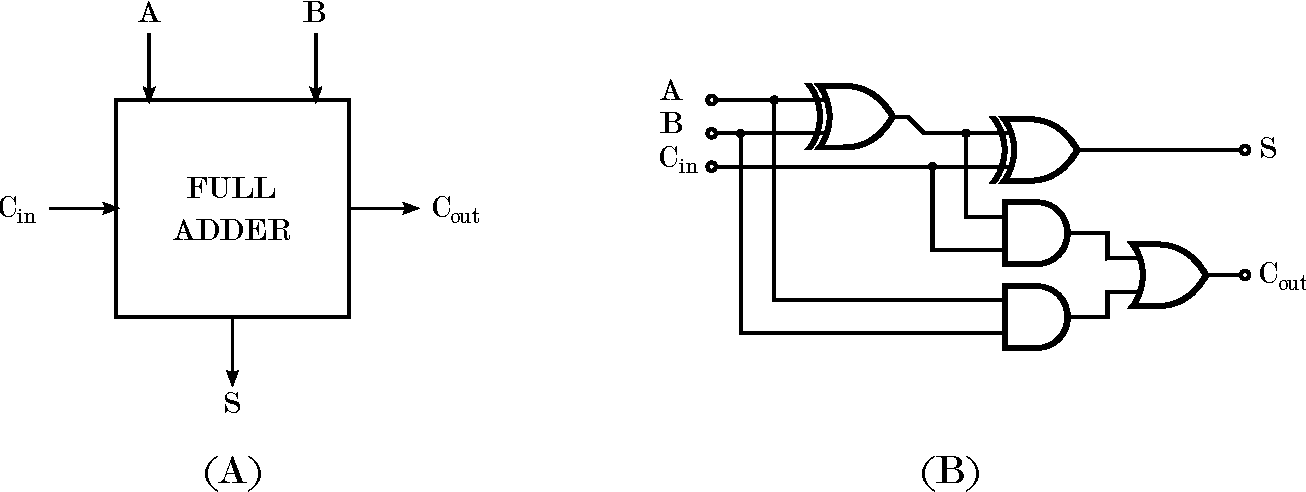
\includegraphics[width=\textwidth]{chapters/figures/fa} 
	\caption{(A) Schematic symbol of a 1-bit full adder. A and B are the operands, Cin is the carry-in while Cout and S are the carry-out and the sum, respectively. (B) Logic diagram of the 1-bit full adder.}
	\label{fig:fa}  % here is the figure label
	\end{figure}

The truth table of the one-bit full adder is shown in table \ref{tab:1}. % here is the reference to the table below

% Below is an example of how to create a simple table. You can create a reference (using \ref{table_label}) to tables too if you give them a label.

	\begin{table}[ht]
	\centering
	\begin{tabular}{ccc}
	\toprule
	A B Cin & S & Cout\\
	\midrule
	0 0 0 & 0 & 0\\
	1 0 0 & 1 & 0\\
	0 1 0 & 1 & 0\\
	1 1 0 & 0 & 1\\
	0 0 1 & 1 & 0\\
	1 0 1 & 0 & 1\\
	0 1 1 & 0 & 1\\
	1 1 1 & 1 & 1\\
	\bottomrule
	\end{tabular}
	\caption{Truth table of a 1-bit full adder.}
	\label{tab:1} % here is the table label
	\end{table}
	
From the truth table we can easily derive the logic equations that describe the full adder:

% Below is an example of how to write equations.

	\begin{equation}
	S = A \oplus B \oplus C_{in}
	\label{eq:1}
	\end{equation}

	\begin{equation}
	C_{out} = AB + C_{in}( A \oplus B)
	\label{eq:2}
	\end{equation}
	
\subsection{Area and power estimation}

A simple Bash script has been written to automatise the calculus of area and power starting from the layout of the circuit. The script takes in input the SVG (which is the primary Inkscape's format) description of the layout and it extracts all the necessary information. The output of the script is a .txt file containing different data.\\
The output text file of the full adder is reported below.

\verbatiminput{chapters/files/planar_FA_area_power.txt}  

% The command \verbatiminput allows you to import the text (e.g, some code or the output resulting from running a program or a script) written in a file.
% You can also include some text in this way:
%	\begin{verbatim}
%		text here
%	\end{verbatim}

% Below is shown how to create an itemize. An alternative to itemize is enumerate that allows you to generate a numbered list. It is used in the same way as itemize:
%	\begin{enumerate}
%		\item bla1
%		\item bla2
%		\item bla3
%	\end{enumerate}

To summarize, the planar full adder is characterized by:
\begin{itemize}
\item Delay = 3 clock cycles;
\item Area = $2.7\ \mu m^2$;
\item Power = $10.53\ \mu W$.
\end{itemize}
	
\section{Ripple Carry Adder}

A Ripple-carry adder (RCA) is a more complex adder composed by a cascade of more full adders. It is used to add N-bit numbers and its name derives from the fact that the carry propagates from a full adder to the next one.\\
\dots \dots \dots \\
\dots \dots \\
\dots
%%%%%%%%%%%%%%%%%%%%%%%%%%%%%%%%%%%%%%%%%%%%%%%%%%%%
% This will help you in writing your homebook
% Remember that the character % is a comment in latex
%
% chapter 1
\chapter{Introduction}
\label{Introduction}

%%%%%%%%%%%%%%%%%%%%%%%%%%%%%%%%%%%%%%%%%%%%%%%%%%%%%%%%%%%
% you can organize a chapter using sections -> \section{Simulating an inverter}
% or subsections -> \subsection{simulating a particular type of inverter}

%%%%%%   First section
    \indent In this short section the main concepts of the architecture are explained along with the related components.
    Additionaly, the added features which make up the Pro version of the DLX will be introduced along with related conceptual diagrams and schematics. 
    Lastly, the chapter will conclude with a mention on how the rest of the documentation is organized. 

\section{DLX Overview}
    The DLX we implemented consists in the computation and propagation of 32 bit instructions. 
    At a given time instant, multiple instructions of a partyicular assembly program are processed as this processor is constructed with a pipeline methodology.
    In particular, the stages of the pipeline for each instruction are given below:
    \begin{enumerate}
        \item Instruction Fetch;
        \item Instruction Decode;
        \item Execution;
        \item Memory;
        \item Write Back;
        \end{enumerate}
	\indent Furthermore, there are three fundamental block of the implemented DLX which are involved during the pipelined execution of the program:
	\begin{enumerate}
        \item Datapath Unit;
        \item Control Unit;
        \item Hazard Unit;
        \end{enumerate}
		These components are explained in the following subsections of this chapter.
	\subsection{ The Datapath Unit }
    \indent The inclusion of the pipeline serves to increase the throughput of the overall program serving to reduce idle times of the processor. 
    The pipeline mechanism is noted most clearly in the datapath and control unit which are the fundamental hierierchical components of the processor.
    In Figure 2.1 the datapath with a pipelined mechanism is depicted. The figure also shows also some external input signals which are entering the datapath. 
	These are control signals which come from another component called the Control Unit which sends appropriate control bits to the datapath depending on the instruction to be executed.
	Another important note about Figure 2.1 is that it depicts 2 memories, the instruction memory (IRAM) and the data memory (DRAM). These two memories
	are external components to the datapath and only interface it. Respectively, they serve an important role in the instruction fetch phase and memory phase of the instructions described later on.
    \begin{figure}[h!]
        \centering
        \includegraphics[scale = 0.15]
		{chapters/figures/DataPathUpdate}
        \caption{DLX datapath component}
        \label{fig:datapathPic}
        \end{figure}

	\subsection{ The Control Unit and Hazard Unit }
	The Control Unit and Hazard Unit are side components which serve to control. Moreover, the control unit is constructed to give orders to the
	datapath about which instructions need to be executed but it gives such orders alertive to possible hazards which could be detected by the Hazard Unit. They will be discussed in a following chapter of the document.

	\section{Pro Version Features}
		The presented DLX has the following capabilities:
		\begin{enumerate}
			\item Extended Instruction set Architecture;
			\item Advanced Arithmetic Logic Unit;
			\item Extra component, the hazard unit;
			\end{enumerate}

			\newpage
		\subsection{ Extended Instruction set Architecture}
		The processor is able to run 50 instructions all listed in this section:
		\begin{enumerate}
			\item \textbf{RTYPE instructions}: ADD, SUB, AND, OR, SGE, SLE, SEQ, SNE, SRL, SRA, SLL, XOR, SLT, SGT, XNOR, NAND, NOR, ADDU, SUBU, SGEU, SGTU
			\item \textbf{ITYPE instructions}: NOP, ADDI, SUBI, ANDI, ORI, BEQZ, BNEZ, LDW, STW, XORI, SGEI, SLEI, SLLI, SNEI, SRLI, SEQI, SRAI, SLTI, SGTI, ADDUI,
			SUBUI, XNORI, NORI, NANDI, SGEUI, SGTUI, JR
			\item \textbf{JTYPE instructions}: JMP, JAL
			\end{enumerate}
		The datapath, control unit and hazard unit are able to process additional instructions with respect to the basic set of instructions.
		some of the additional instructions involve the ability to distinguish signed operands with unsigned for some operations, extra logical functionalities, more compare functionalities, and the ability
		to jump to an address stored in a particular register.

		\subsection{ Advanced Arithmetic Logic Unit }

		The inner components of the arithmetic Logic Unitc Unit are of advanced type. it is composed of a pentium 4 Carry LookAhead Spare Tree for more efficient addition and subtraction operations. 
		In addition, the logicals have been designed d with the T2 Logic methodology. The relevant schematics of the introduced inner components of the arithmetic logic unit are analyzed in Execution Unit section of the report

		\subsection{ Extra component, the Hazard Unit }

		This additional component is inside the DLX and it is able to make the distinguishment of the following type of hazards:

		\begin{enumerate}
			\item Read After Write Hazards 
			\item Control hazard for branch instructions
			\item Jump detection
			\end{enumerate}

		These hazards will be detected and given to the control unit which will actuate the stall for the datapath. More information on the hazard unit will be given later on in the report.

		\section { Structure of the report }

		The structure of this documentation consists in the thorough analysis of the components in the datapath based on the pipeline stages. 
		Consequently an analysis on the implemented Control Unit and Hazard Unit is exposed explaining also their exhange of informatio.
		Lastly, an insight on the synthesis and physical design process is made available. In the next section we analyze the datapath starting from the components
		dedicated to the Fetch Stage.


%%%%%%%%%%%%%%%%%%%%%%%%%%%%%%%%%%%%%%%%%%%%%%%%%%%%
% This will help you in writing your homebook
% Remember that the character % is a comment in latex
%
% chapter 3
\chapter{Fetch Stage}
\label{FetchUnit}

The fetch part of the datapath serves to do the operation of obtaining the current instruction.
from the external Instruction Memory (where the program is stored) to then feed it to the subsequent unit of the datapath which decodes the bits.
In this small section there will be the analyzation of the components of the datapath in this respective unit along also the external Memory from which the Instruction Register acquires the data.


\section{Datapath Related Components}

\subsection{ Program Counter Register }
First of all there is the Program Counter Register whose purpose is to store the current address of the instruction inside the Instruction Memory from
which the instruction is fetched. Additionally, this register is synchronous reset and enable to the clock. At reset time, the PC register stores the 
all zero value, meaning that there will always be the fetching of the instruction at the adress 0x00000000 at start up. 
Another important remark is about the signal of input of the PC depends on the outcome of two combinational multiplexers. One multiplexer decides to
feed through the address of the next instruction or the address coming from the output of the ALU in the execute stage. This decision is made on the basis
of a branchStatus signal determined during the Execution Stage, which takes value 1 when a jump or branch needs to be performed.
As a second criteria, we included the second multiplexer to decide if it is needed to stall the PC register or not. This action depends on whether the hazard unit
external to the datapath detects a hazard in the program. In such case it sends a selection signal for this multiplexer set to 1, for making the Program 
counter register assume the same address value in the subsequent clock cycle, so that a stall in the pipelined is formed halting the program.

Additionally, in order to compute the address of the subsequent instruction of the program, a ripple carry adder is used with a fixed operand of one added
to the next instruction.

\subsection{ Instruction Register }

This is the second important register which will store the value of the fetched instruction from the Instruction Memory. like the program counter register,
it has a synchronous enable and a synchronous reset sensitive to rising edges of the clock. The output of this register is propagated and used for the nex important stage,
the decode stage which is explained in the following chapter. 

\subsection{ Next Program Counter }

This important register is placed for the propagation of the subsequent instruction address for the following pipe stages. This way, if the instruction
that was fetched is a jump or a branch, it will be able to compute the address of the jump later on in the execution stage.

\section{External Instruction Memory}

The instruction memory is the memory where all the instructions of the program are stored and it is the component from where the Instruction Register fetches the 
instruction. Upon the presence of an active high reset signal, it loads in a raw format all the thirtytwo bit instructions composing the program. While the reset is zero,
on the basis of the adress that is felt at its input it outputs the associated instruction for the Instruction Register.

In Figure 3.1 is a conceptual drawing which is made to visualize the structure of this component more clearly. the main criterias to consider are that this
memory will always store the first instruction of the program at the all zero address. The second feature of the memory is that it stores the whole instructions
in a row of the memory, this leads to the reason why the addresses are incrememnted by one instead of four, and also it is the reason why the
ripple carry adder adds one instead of four for computing the subsequent instruction's address. We designers made this decision for the purpose of easily creating the
raw memory files while testing the datapath in the early stages. Also another small advantage of this choice is that the minimum required depth of the memory in thi way is exactly the amount
of instructions of the assembly program

\begin{figure}[h!]
    \centering
    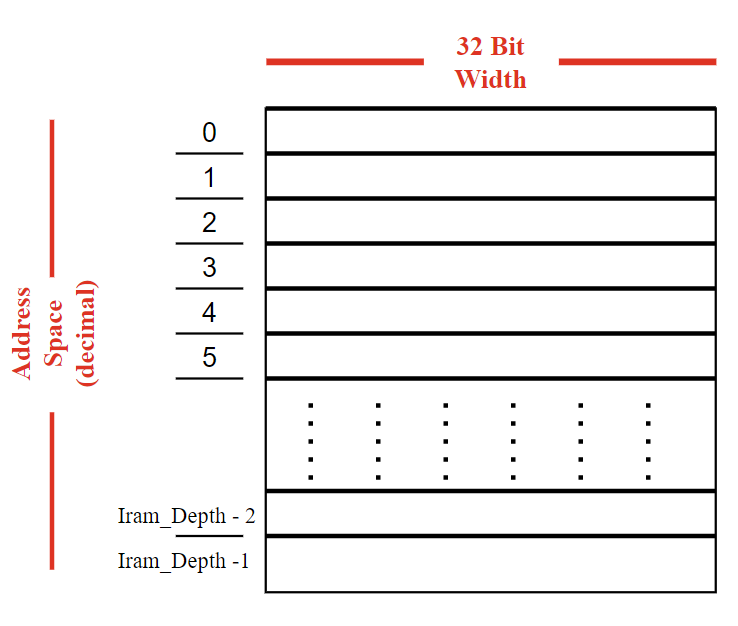
\includegraphics[scale = 0.45]
    {chapters/figures/IRAM}
    \caption{Instruction Memory with addresses separated by one as offset}
    \label{fig:IRAMpic}
    \end{figure}



%%%%%%%%%%%%%%%%%%%%%%%%%%%%%%%%%%%%%%%%%%%%%%%%%%%%
% This will help you in writing your homebook
% Remember that the character % is a comment in latex
%
% chapter 4
\chapter{Decode Stage}
\label{DecodeUnit}

In this part of the datapath the instruction that was previously fetched is broken down and given to several components.
This part of the datapath contains more circuitry with respect to the fetch unit:

\begin{enumerate}
    \item Sign Extender Module and 4to1 multiplexer;
    \item Register File;
    \item Pipe Registers for subsequent execution phase;
    \end{enumerate}

\section {Sign Extender Module and four to one multiplexer}

    The sign extender module is designed with the final goal of interpreting correctly the immidate bit field stored in an immidiate type or jump type instructions.
    In fact, as the implemented DLX gives the possibility to distingush operations for unsigned and signed operations, this combinational block 
    gives the possibility to extend the most significant bit of the immediate field of the immediate type instruction (sixteenth least significant bit) to the the other sixteen bits. 
    The same is done for the immediate field of the Jump-Type instructions (this time containing a twentysix bit width instead of sixteen).
    The reason for this choice is because the DLX wires all have thirtytwo bit width, hence we must extend the original immidiate value of the instruction accodingly.
    Furthermore, there are four possible possibilities of interest that could be presented: 
    \begin{enumerate}

        \item an Immidiate-Type instruction interpreting the immediate field as signed: in this case depending on the Most significant bit of the immediate
        bit field, the sixteen additional most significant bits will be either zero, or one. in this scenario we are extending a sixteen bit immediate to a thritytwo bit value.
        
        \item an Immidiate-Type instruction interpreting the immediate field as unsigned: in this case regardless of the Most significant bit of the immediate
        bit field, the sixteen additional most signinfiant bits will be zero. In this scenario we are extending a sixteen bit immediate to a thritytwo bit value.
     
        \item a Jump-type instruction interpreting the immediate field as as signed: in this case depending on the Most significant bit of the immediate
        bit field, the six additional most signinfiant bits will be either zero, or one. in this scenario we are extending a twenty six bit immediate to a thritytwo bit value

        \item a Jump-type instruction interpreting the immediate field as unsigned: This scenario is not implemented in the datapath as the jump instructions always consider
        a signed value of the immediate field. However for a future improvement of the DLX it could be used for a type of jump instruction that can only jump forward.

        \end{enumerate}

    All these scenarios are performed in parallel in the decode unit, and thanks to a four to one multiplexer, the correct specific scenario is selected for obtaining
    the appropriate extension. Furthermore, the selection bits of the multiplexer individuating the correct extension scenario come from two control bits from the control unit.

\section {Register file}

    The Register file of the DLX consists of thirtytwo registers. The register at address zero is always zero by convetion while the thirtysecond
    register is only utlized for the storing of the return address when executing a jump and link (jal) instruction. A main schematic block is shown in Figure 4.1 .

\begin{figure}[h!]
    \centering
    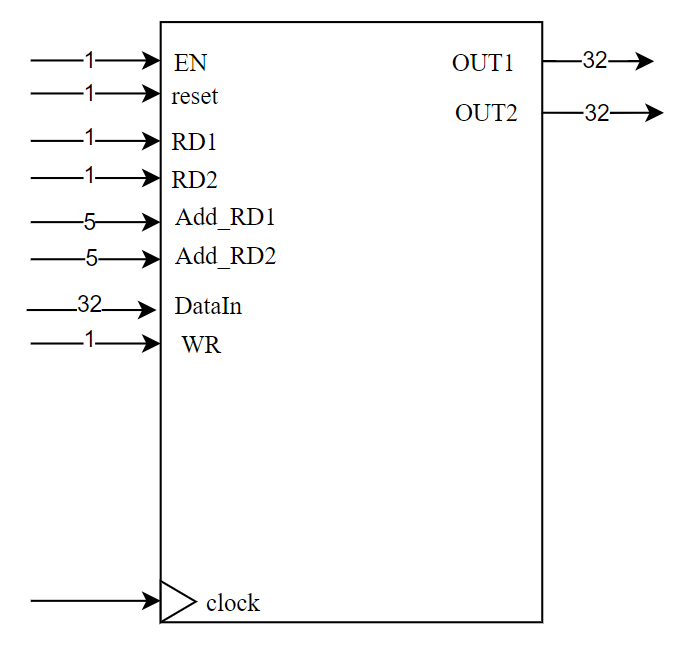
\includegraphics[scale = 0.45]
    {chapters/figures/RegisterFile}
    \caption{Register File Schematic }
    \label{fig:RFpic}
    \end{figure}

        \subsection{Reading Methodology}
        The register file has two read ports. The reading is done asynchronously this way it is easier for the register file to obtain the proper
        addresses of the register for which the reading is performed. On the basis of the RD1 and RD2 single bit port signals, the ports for reading can be activated.
        After receiving the proper addresses from the Instruction register bits, the values of the registers are made available at the OUT1 and OUT2 ports respectively.

        \subsection{Writing Methodology}
        The writing methodology is synchronous to falling edges of the clock cycle. This is done to avoid the issue of metastability.

        In fact if the register file were to sample the DataIn port at the rising edge of the clock cycle, since the control unit sets the write port
        at rising edges of the clock cycle, the register file would understand as if the write port bit is zero hence leading to an incurrect behavior. Furthermore, 
        this is the reason why the write process is sensitive to the falling edge od the clock.
        About the reset, it is sensistive to the falling edge of the clock and when it is active high. At the start up of the processor, thanks to the reset all the
        registers of the register file as set to inital value zero.

\section {Decode Pipe Registers}

    There are many Pipeline registers which store relative information all of them having syncronous enabling and resetting at the rising edge of the clock cycle:

    \begin{enumerate}

        \item NPC1: This pipeline register is needed as it needs to be propagated to the Execution unit in case there is the need to compute an address 
        because the instruction of interest is a branch or a jump.
        \item RegisterA and RegisterB: These registers store the output of what was read from the asynchronous reading of the register file. If in the decode
        stage there is a Register type instruction both of these registers will be filled with useful values to be later used in the Execute stage.
        \item ImmREG : This register stores the final extended form of the immediate value that was chosed from the four to 1 multiplexer described earlier in this section.
        \item RT and RD Registers: the need of this register is important do the fact that there is a variation  in position of the destination register field of an instruction;
        in fact for immediate type instruction the destination register address is stored in bit field range [20 downto 16]. While for the Register type instruction it is located
        in the bit range [15 downto 11] of the instruction. Hence in the decode both information are stored, to then decide based on the instruciton type which is the correct address
        for writing back to the register file.
        \item IR1: This will keep the instruction that was analyzed during the decode stage also in execute. This register was implemented for viewing the waveforms
        while debugging the processor's course of actions.

        \end{enumerate}
    
\chapter{Execution Stage}
\label{ExecutionUnit}

After the Decode stage there is the Execution unit which consists of  computation of the acquired information during the earlier decode stage.
This part of the datapath has a very important component called the Arithmetic Logic Unit which is utilized for perforing various operations depending on the specific instuction.
This part of the datapath also contains the important digital circuitry used for analyzing branches and jumps, needed to understand what address to place 
at the content of the program counter in the fetch phase for the next clock cycle. Lastly a brief description of the pipeline registers related to this stage is provided.

\section{ The Arithmetic Logic Unit }
The DLX has these following arithmetic operations:
\begin{enumerate}
    \item T2 Shifter;
    \item Pentium 4 Adder;
    \item Comparator ;
    \item T2 Logical ;
    \end{enumerate}

Furthermore Figure 5.1 depicts the black box structure of the Arithmetic Logic Unit. There is a final four to 1 multiplexer which selects which results
needs to be given as the ouput of the operation. This selection depends on the particular instruction's predefined control bits that are given as output from the
control unit. The operands A and B from which the ALU performs the introduced operations are finalized thanks to two independent multiplexers. One multiplexer
chooses if the Operand called Operand A needs to feedthrough the Next Program Counter Value, or the Value which came from OUT1 port of the register file. On the other side,
the second multiplexer chooses if the second operand called operand B should be the value read from port OUT2 of the register file, or the Immediate field. There are 2 control
bits which make the decision as they are the selection signals of these multiplexers.

\begin{figure}[h!]
    \centering
    \includegraphics[scale = 0.55]
    {chapters/figures/ALUinternalUpdate}
    \caption{Schematic of internal Black Box ALU components }
    \label{fig:insideALU}
    \end{figure}

\newpage

\subsection{T2 Shifter}
 The shifting methodology used is the same one used as the T2. This means that the shifting is performed on the basis of the following three levels:

 \begin{enumerate}
    \item First Level: formation of all the masks that are to be applied in the next levels of the computation
    \item Second Level: on the basis of the formed masks during the first level and the amount of shifting that is to be done,
    the mask which is most similar to the real amount that needs to be shifted is selected. Alternatevely it can be said that this level is broad
    shifting operation
    \item Third Level: starting from the output of the shifted version from the Second Level of computation a fine grained level shifting is done at this level,
    which means that the final shifted result of the shifting operation is finally calculated.
    \end{enumerate}

    Figure 5.2 rapresents the concepts that are above discussed (all though applied assuming that the input is of 64 bits).

    \begin{figure}[h!]
        \centering
        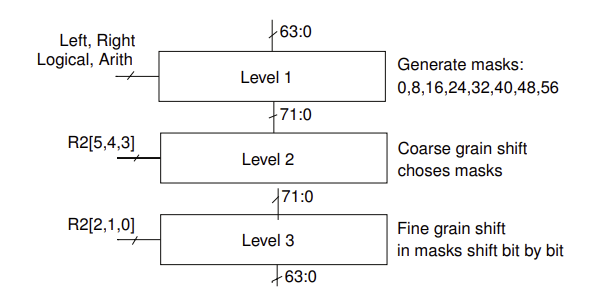
\includegraphics[scale = 0.8]
        {chapters/figures/T2Shifter}
        \caption{Black Box schematic of the T2 Shifter}
        \label{fig:T2Shifter}
        \end{figure}
    

    \subsection{ The Pentium 4 Adder}
    It is an efficient adder whose implementation is to minimize the critical path by making the bits of the operands that are being added or subtracted less vulnerable on 
    the carry bit propagation during the addition. Specifically, the adder is composed of two main blocks:

\begin{enumerate}
    \item The Carry Look Ahead Sparse Tree: It is a tree like structure formed of interconnected Propagate and Propagate-Generate blocks included for relying less on the dependency of the carry out done
    formed in a previous stages, for reduction of the critial path.
    \item The Carry Select Sum Block: similar to the Carry Look Ahead Adder concept; it is formed of a series of stages made of a specific predefined amount of concatenated full adders.
    Each stage has two parrallel chains of full adders  which perform respectively the addition on the hypothesis that the carry in bit is zero and one respectively.
    Then, the correct output of the addition between a particular subset of bits of the operands is chosen on the basis of the actual local carry produced by the sparse tree block described previously.
    
\end{enumerate}

    Summarizing, the adder/ subtractor module is implemented in a more efficient manner this way do to the fact that the addition of the particular subset of bits of the operands
    are all done in parallel unlike for instance the basic ripple carry adder model. Additionally, each set of ripple carry adders in the Carry Select Sum Block does not have to 
    wait for the carry out from the previous stage to perform the computation. Meaning that thanks to the Sparse tree, the addition/subtraction of the Pentium4 adder is more efficiently parallelized with respect to the addition
    performed by the Carry Look Ahead Adder model.

    Figure 5.3 depicts the block schematic of the described high level blocks which make up the pentium 4 adder module.

    \begin{figure}[h!]
        \centering
        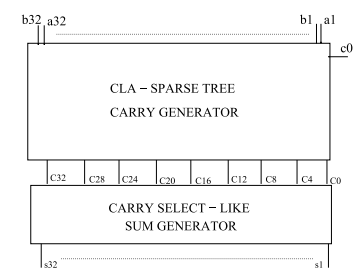
\includegraphics[scale = 1]
        {chapters/figures/Pentium4Adder}
        \caption{Black Box schematic of the Pentium 4 adder.}
        \label{fig:Pentium4Adder}
        \end{figure}

    \subsection{ The Comparator }
        The implemented comparator is constructed using the ouput of the present pentium four adder. Moreover, if two operands need to be compared,
        they will be firstly given to the pentium 4 block which will perform a subtraction. The comparator block will analize the carry out obtained from the results
        along with a flag bit called Z used set to one if the result of the subtraction is zero.
        Additionally the implemented comparator is able to perform a dual kind of operation in case the operands are treated as unisgned instead of signed.
        Figure 5.4 reports the schematic depicting the implementation of the comparator for the operands which are understood as signed.

        \begin{figure}[h!]
            \centering
            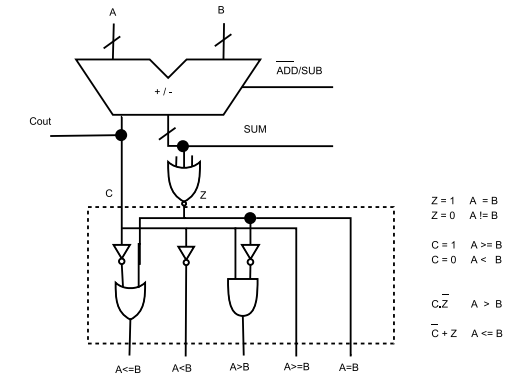
\includegraphics[scale = .6]
            {chapters/figures/Comparator}
            \caption{The Comparator}
            \label{fig:T2Logic}
            \end{figure}

    \subsection{ The T2 Logicals }

    Logical instructions like the AND, OR and many others are performed through the T2 circuitry design. This choice was made as it leads
    to the implementation of a lot of logical operations still while using few gates (meaning less transistors equivalently). The structure is composed
    of four and gates in the fisrt level of the hirierchy. Then, the second level is one additional final and gate doing the and between the outputs of the first level.
    On the basis of the control bits of the dedicated to the execute phase there is the possibility to implement the logical operation of interest.
    Figure 5.5 depicts the circuit methodology of the comparator for the situation in which the .

    \begin{figure}[h!]
        \centering
        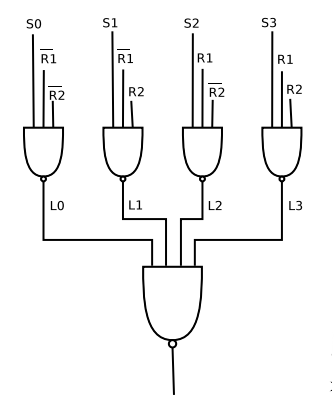
\includegraphics[scale = .6]
        {chapters/figures/T2Logic}
        \caption{The T2 Circuit for Logical Operations}
        \label{fig:T2Logic}
        \end{figure}

    For more details on the components specified above, chapter four from the Microelectronic Systems Lecture notes provides a more thorough analysis.
\newpage

\section{ Branch and Jump Related Circuitry }

The DLX sends out the selection signal for jumping in the fetch stage in the execution stage. Similarly, in case of a branch instruction,
the DLX determines whether the branch needs to be taken or not in the execution stage. the mechanism implemented for knowing if the branch and
jump need to be taken is composed of three multiplexers distributed hirierchically. In the first level of the hirierchy, there are two multiplexers.
one of them receives 1 and a signal called 'cond' (wich is the flag indicating if value stored the "REGA" pipe decode register is zero or not), and the other multiplexer has zero as first input 
and a signal called 'notCondIn' (which is the inversion of the of the CondIn signal ). The output of these two multiplexers are controled by one bit of the 
control unit which is one if the instruction is a Branch instruction, while when it is zero the instruction at analysis is not a branch. 
In the  second level of the hiriechy of the multiplexers there is one multiplexer which decides how to interpret the input it has (if it needs for instance
to branch due to an inequality of zero or due to an equality of zero.) Also for this second level of the multiplexer hiriechy there is a dedicated control bit from the  control unit.
Figure 5.6 depicts the multiplexer hiriechy that was discussed along with a table associating the control bits of interest to the various intructions

\begin{figure}[h!]
    \centering
    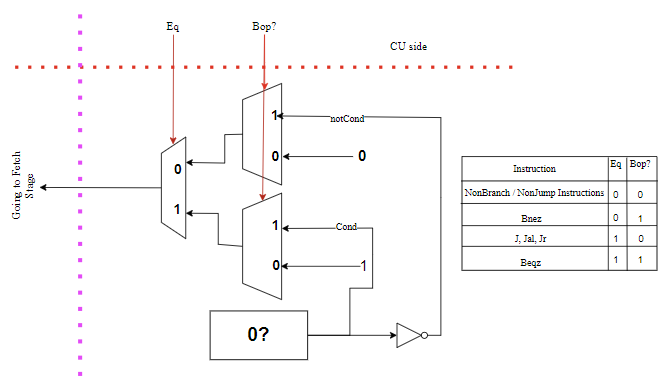
\includegraphics[scale = 0.8]
    {chapters/figures/BranchAndJumpDecision}
    \caption{The two level hirierchy of the multiplexers with an explenation table}
    \label{fig:BranchAndJumpDecision}
    \end{figure}

\section{ Execution Pipe Registers }

The execution stage has the following Pipe Registers:
\begin{enumerate}
    \item ALUOutReg: in this pipe register the result of the alu operation is stored in the case that for instance the result needs to 
    be written back to the register file during the write Back Stage
    \item NPC2: this pipe register is needed for propagating the NPC address in the eventual case that the instruction of interest is
    a jump and link instruction. In such case there will be the need to store this address in the the thirtysecond address of the register 
    file during the write back, hence the reason we need to save it.
    \item ForMemStRegister: this register is needed in the case the instruction is of store type. Thanks to this register the subsequent stage (the memory stage) will
    be able to obtain the correct value to store in the external DRAM memory.
    \item RDdestReg: In the execution stage the final decision on which is the correct destination address for writing is made (between rd or rt depending on if the instruction is immediate or register type).
    Hence this register is needed to store this finalized address so that during the future Write Back stage, the writing of the result is performed in the correct location of the register file
    \item IR2: needed for help during the debug process while checking the waves on Modelsim while testing the single datapath unit.
\end{enumerate}

\chapter{Memory Unit}
\label{Memory Unit}
Memory Unit is the fourth stage of the pipeline.It is composed by the Data Memory and the pipeline registers. There are five different registers:
\begin{enumerate} 
    \item Three out of five are used to pipeline the destination address, the npc and the instruction.
    \item One is used to pipeline the result of the ALU from the execution unit.
    \item The last one is used to take the output of the Dram in the memory unit.
\end{enumerate} 
\section{Dram}
Dram contains the data for load/store instructions and the values available at the start of the execution are initialized during the reset phase thanks to "DMEM\_init\_file.mem" (easier debug for load and store).
The correct instruction is executed based on RW signal(read/write signal) that it is sent by the Control Unit.
\subsection{R/W process}
During the process,  as inputs arrive an unique address, the data pipelined from the execution unit (RegB), RW and EN from the Control Unit. The read operation starts 
when EN='1' and RW='1' (load instruction) instead for write operation when EN='1' and RW='0' (store instruction), both synchronous with the falling edge of the clock.
The output ,in case of read, is sent to the pipeline register LMDreg in memory unit to be pipelined to writeback.
\chapter{Writeback Unit}
\label{Writeback Unit}
Writeback Unit is the fifth stage of the pipeline and it is composed by three different multiplexers, controlled, using SEL signals, by three different bits of the control word sent by the CU.
\begin{enumerate} 
    \item The first one takes as inputs the output of the alu pipeline register and the output of the dram pipeline register. This mux is used to choose between a value obtained
    from the DRAM with controlwordbit1='1' (load instruction) or from the ALU with controlword1='0'.
    \item The second takes as inputs the output of the first multiplexer and the output of the NPC3 pipeline register. In this case , it is used to choose which value must be saved
    in the register file, NPC3 with controlwordbit2='1' in case of jal instruction or the value from the previous mux controlword2='0'.
    \item The last one is linked to the second mux because it chooses 31 as value when it is a jal and so the value of NPC3 must be stored in r31 with controlword3='1', in the other cases
    the value of the address destination pipeline register with controlwordbit3='0';
\end{enumerate}
\chapter{Control Unit}
\label{Control Unit}
The Control Unit is an Hardwired Control Unit and controls the Datapath generating the proper controlword based on current instruction in the proper clock cycle. It is divided in different parts:


\begin{figure}[h!]
    \centering
    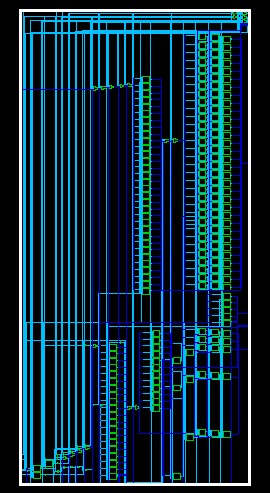
\includegraphics[scale = 0.30]
    {chapters/figures/CU_highlevel}
    \caption{CU}
    \end{figure}


\begin{enumerate} 
    \item Look-Up Table: it contains all the control words linked to the instrunctions
    \item Three processes that work one after the other:
    \begin{enumerate}
    \item The first one takes the main input of CU (IR\_In) and consider the relative opcode and func of the instruction which are used by the second process.
    \item The second one takes the opcode and func of the first process (checking if RTYPE,ITYPE,JTYPE) and use them to take the correct control word from the look-up table.
    \item The last one works to pipeline the control words in the right way (as an Hardwired Control Unit do) and there is also the pipeline of the instructions that it is used for the Hazard Unit.This process, also, takes as inputs the three hazard signals from the HU to flush the pipeline putting NOP in the decode stage and execute stage for branch hazard or putting NOP in decode stage for jump untill the new PC or putting NOP in execute stage and maintaining the same cw (and istruction)in the decode stage for raw hazard.The flush of the pipeline depends on where the hazard is taken (specified in the HU chapter), it lasts one or more cycles. 
    \end{enumerate}
\end{enumerate}
\subsection{Control Word}
The main job of the Control Unit is to generate the right control word using the look-up table. Each control word is saved in the file "INSTR\_CODES.vhd" with all the opcode and func of the instructions.
The bits are divided for Decode Unit, Execution Unit, Memory Unit, Writeback Unit and they are pipelined during the cycles to be used in the correct moment of the pipeline to activate the useful components of the datapath.


%\chapter{Physical Design}
\label{physical_design}

% Below is shown how you can insert a figure. If you give a label to the figure, you can refer to the figure using \ref{figure_label} as shown above. 
	\begin{figure}[ht]
	\centering
	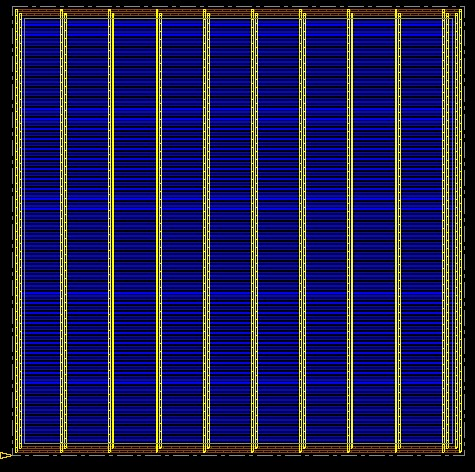
\includegraphics[width=\textwidth]{chapters/figures/4.horizontal_lines.jpg} 
	\caption{Power grid distribution}
	\label{fig:power_distribution}  % here is the figure label
	\end{figure}

This is the final step, in which the layout of our DLX design can be generated, using the \textbf{Innovus} tool, provided by Cadence.
The entire procedure is composed of various steps, from Floorplanning to Cell Placing and signal Routing.

To start creating the floorplan, Innovus needs a verilog post-synthesis netlist, a \textit{.lef} file that has references to the library of cells and other data which is
provided in the project files. In this step the area dedicated to the chip core is computed, along with the power supply rings around it.
%% put figure
Next, the power rings for \textit{Vdd} and \textit{GND} are inserted in the model and on the layout corner, the vias to connect the metal layer are placed as well. To avoid congestion, M9 and M10 metals are chosen for the rings.
The rings are then connected using vertical stripes and horizontal lines, to better distribute power into the center of the chip.
Power Grid Placement is shown in Figure \ref{fig:power_distribution}.

\begin{figure}[ht]
	\centering
	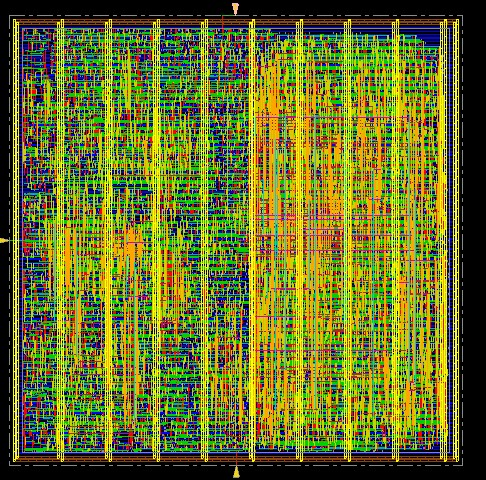
\includegraphics[width=\textwidth]{chapters/figures/7.Post_CTS_optimization.jpg} 
	\caption{Post CTS Optimization}
	\label{fig:CTS_OPT}  % here is the figure label
	\end{figure}

\section{Placement and Routing}
In the Placement phase, the cells are placed, along with I/O pins. Post CTS (Clock-Tree-Synthesis) optimization is performed before routing.
The result is shown in Figure \ref{fig:CTS_OPT}.
Before the routing phase, it is important to complete the placement filling free spaces in the layout with \textit{Filler Cells}, to maintain the continuity of the N+ and P+ wells.

The final step is the \textbf{Post routing optimization}, in which the design is optimized in order to achieve the timing constraints.
Now the design is complete and a final verification can be performed to see if there are violations with respect to design rules and connectivity.

\begin{figure}[ht]
	\centering
	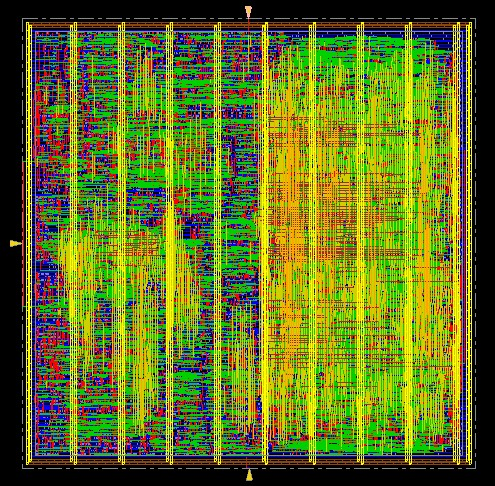
\includegraphics[width=\textwidth]{chapters/figures/9.Post_PostRouteOPT.jpg} 
	\caption{Final layout}
	\label{fig:final_design}  % here is the figure label
	\end{figure}

The final layout is shown in \ref{fig:final_design}










\chapter{Hazard Unit}
\label{Hazard Unit}

The Hazard Unit is used to detect 3 different type of hazard: 
\begin{enumerate} 
    \item Raw Hazard in which the pipeline stall to wait the value to read
    \item Jump Hazard 
    \item Branch Hazard
\end{enumerate}

To detect these hazards , the HU works on two processes , executed one after the other.
\begin{enumerate} 
    \item First process: It works on the inputs coming from the CU (IRID,IREX,IRMEM). It uses the pipeline and the opcode of the instruction (ITYPE,JTYPE,RTYPE) to take the correct registers used by the instructions (RS1,RS2,RD).
    This analysis creates also a pipeline of the registers to take in to account in which position of the pipeline they are in the clock cycle.
    \item Second process: It is the process used to detect the hazard and it is divided in 2 main part:
    \begin{enumerate}  
        \item In the first part simply there is the detection of a jump/jr/jal in the decode stage (for jr there is also a control on the register used that it could create raw hazard).
              Also the detection of the branch in the execute stage thanks to the result (Branchstatus) given by comp4Branch in the Datapath.In the if of jump/jr/jal there is a AND branchstatus because of a problem
              caused by a branch followed by a jump that created error.
        \item Second part: It is used to detect raw hazard between the destination registers in execution-memory-with the source registers of the instruction in decode. All the possible combination are considered (ITYPE,RTYPE different source registers and destination registers positions)
    \end{enumerate}
\end{enumerate}

When a hazard is detected a signal colled PC_sel is rised to stop the pc (except for branch) and have stalls in the pipeline with the insertion of NOP in the correct position for Execution stage and Memory stage made by the CU.After the useful stalls , the hazard signal and the PC_sel go at 0 and the code restart its correct pipeline.


% \input{./chapters/chap_name}
% and so on
%
%%%%%%%%%%%%%%%%%%%%%%%%%%%%%%%%%%%%%%%%%%%%%%%%%%%%%%
%    
% HERE IS WHERE YOU INCLUDE YOUR APPENDICES (IF ANY)
%
\appendix
%%% Appendix A
\chapter{Synthesis Reports}
\label{appendix1}

\section{Power Report}
	\lstinputlisting{appendices/files/CFG_CPU_clk_1.5ns_power.rpt}

\section{Timing Report}
	\lstinputlisting{appendices/files/CFG_CPU_clk_1.5ns_timing.rpt}

% \lstinputlisting is an alternative way to import text or code from an external file. In this example the behavioural VHDL description of an adder contained in the file adder.vhd is imported. 
% Note that you can set the language of the code that you want to import (VHDL in this example). When you set the language you will see the keywords of that specific language highlighted in your output pdf file.
%You can set a lot parameters: for some examples take a look at the chapter 'How to document the project' that can you find in DLX_Project.pdf.
% \input{./appendices/appendix2}
% and so on
%
%%%%%%%%%%%%%%%%%%%%%%%%%%%%%%%%%%%%%%%%%%%%%%%%%%%%%%

\end{document}